\newpage
\section{The Query Model}

\textcolor{red}{TODO: Formal description of the qeury model\\}

\subsection{Fraud Pattern I - Card Cloning}

A first algorithmic proposal to detect this kind of fraud pattern is the one shown in the algorithm
\ref{alg:check-fraud-1}. Note that $S$ refers to the filter's subgraph and $e_{new}$ is the new incoming edge belonging to the filter, such that it is a opening interaction edge, since in the case it is a closing interaction edge, we do not perform the \text{CheckFraud()}.

\begin{algorithm}[H]
    \small
    \begin{algorithmic}[1]
    \REQUIRE $S$ is the subgraph of edges of the filter (sorted by time)
    \REQUIRE $e_{new}$ is the new incoming opening interaction edge belonging to the filter 
    \STATE $\texttt{fraudIndicator} \gets \texttt{False}$
    \STATE $i \gets |S|$
    \WHILE{$i > 0$ \AND \texttt{fraudIndicator} = \texttt{False}}
      \STATE $e_i \gets S[i]$
      \STATE $\texttt{t\_min} \gets \text{obtain\_t\_min}(e_i, e_{new})$
      \STATE $\texttt{t\_diff} \gets e_{new}.start - e_i.end$
      \IF{$\texttt{t\_diff} < \texttt{t\_min}$}   
        \STATE $\text{createAlert}(e_i, e_{new})$
        \STATE $\texttt{fraudIndicator} \gets \texttt{True}$
      \ENDIF
      \STATE $i \gets i - 1$
    \ENDWHILE
    \end{algorithmic}
    \caption{$\text{CheckFraud}(S, e_{new})$ -- \textbf{initial version}}
    \label{alg:check-fraud-1}
\end{algorithm}

There are some aspects and decisions of this algorithm that are worth to describe:

\begin{itemize}
    \item \textbf{Pairwise detection}. The checking of the anomalous fraud scenario is done doing the check between the new incoming edge $e_{new}$ and each of the edges $e_i$ of the filter's subgraph $S$.
    \item \textbf{Backwards order checking}. The pairs $(e_{new}, e_i)$ are checked in a backwards traversal order of the edge list of the subgraph $S$, starting with the most recent edge of the subgraph and ending with the oldest.  
    \item \textbf{Stop the checking whenever the first anomalous scenario is detected}. Whenever an anomalous scenario corresponding to a pair ($e_{new}, e_i)$, then we stop the checking at this point and emit the corresponding alert. Therefore we do not continue the checking with previous edges of $S$. 
    \item \textbf{Emission of the pair $(e_{new}, e_i)$ as the alert}. The alert is composed by the pair $(e_{new}, e_i)$ that is detected to cause the anomalous scenario. Both edges are emitted in the alert since we do not know which is the one that is the anomalous. On the one hand, it can be $e_i$, which is previous to $e_{new}$, in the case that $e_i$ at the moment it arrived it did not cause any alert with the previous edges/transactions of the subgraph and it causes it now with a new incoming edge $e_{new}$ which is a regular transaction of the client. On the other hand, it can be $e_{new}$, which is the last having arrived to the system, that it directly causes the alert with the last (ordinary) transaction of the card.
\end{itemize}

However, a more detailed study, lead us to a simplification of the initially proposed algorithm to the one shown in \ref{alg:check-fraud-def}. On it we just perform the checking between the new incoming edge $e_{new}$ and the most recent edge of the subgraph $S$, $e_{last}$.

\begin{algorithm}[H]
  \small
  \begin{algorithmic}[1]
  \REQUIRE $S$ is the subgraph of edges of the filter (sorted by time)
  \REQUIRE $e_{new}$ is the new incoming opening interaction edge belonging to the filter 
  \STATE $last \gets |S|$
  \STATE $e_{last} \gets S[last]$
  \STATE $\texttt{t\_min} \gets \text{obtain\_t\_min}(e_{last}, e_{new})$
  \STATE $\texttt{t\_diff} \gets e_{new}.start - e_{last}.end$
  \IF{$\texttt{t\_diff} < \texttt{t\_min}$}   
    \STATE $\text{createAlert}(e_{last}, e_{new})$
  \ENDIF
  \end{algorithmic}
  \caption{$\text{CheckFraud}(S, e_{new})$ -- \textbf{definitive version}}
  \label{alg:check-fraud-def}
\end{algorithm}


In what follows we argument the reason why it is sufficient to just check the fraud scenario among $e_{new}$ and the last/most recent edge of the subgraph and not have to continue having to traverse the full list of edges.

Assume that we have a subgraph as depicted in Figure \ref{img:fp-I-demo}, and that we do not know if there have been anomalous scenarios produced between previous pairs of edges of the subgraph. Name $F_I(y_i,y_j)$ a boolean function that is able to say whether it exists an anomalous fraud scenario of this type between the pair of edges $(y_i,y_j)$ or not. In addition, note that the edges of the subgraph $S$ are ordered by time in ascending order, in such a way that $y_1 < y_2 < y_3$. Finally note that $y_3 \equiv e_{new}$ as it is the new incoming edge and $y_2 \equiv e_{last}$, since it is the last edge / the most recent edge of $S$.

\begin{figure}[H]
  \centering
  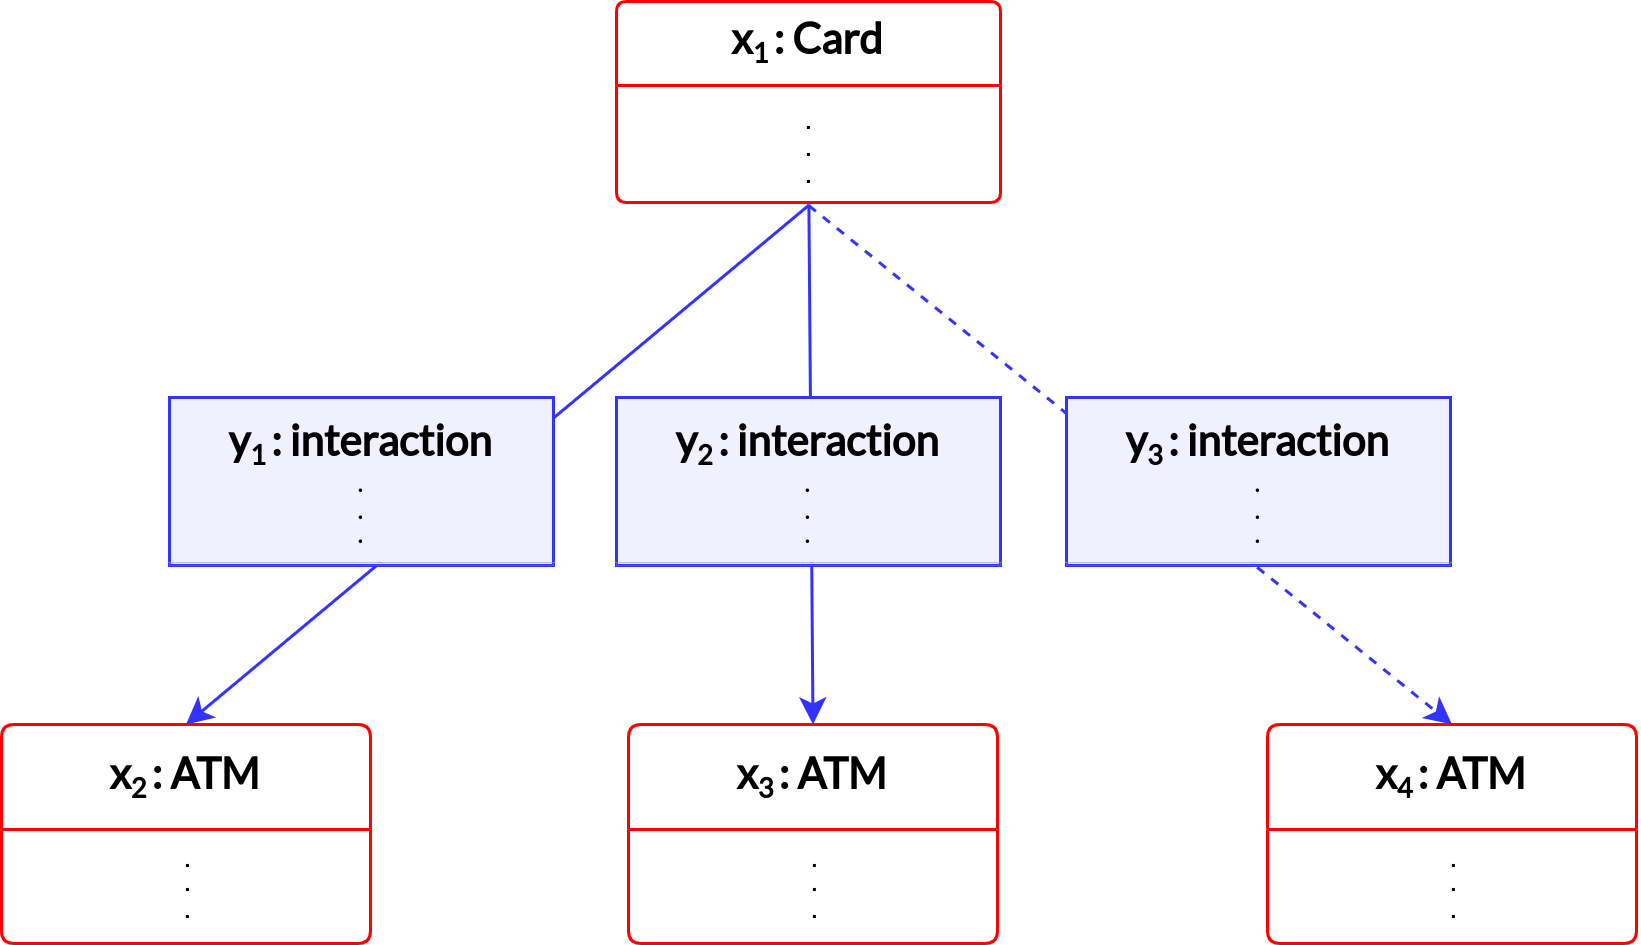
\includegraphics[scale = 0.6]{images/2-QueryModel/fp-I-demo-1.png}
  \caption{Subgraph $S$ of a card -- Fraud Pattern I}
  \label{img:fp-I-demo}
\end{figure}

Note that we can have that:
\begin{itemize}
    \item $F_I(y_2,y_3)$: We emit an alert of this anomalous scenario produced between the pair $(y_2,y_3)$. We could continue checking for anomalous scenarios between $y_3$ and previous edges of the subgraph. However, what we consider important for the bank system is to detect the occurrence of an anomalous scenario in a certain card. Therefore, we consider that, to achieve this, it is enough to emit a single alert of anomalous scenario on this card, and not many related with the same incoming transaction of the same card.
    \item $\neg F_I(y_2,y_3)$: We analyze whether it would be interesting or not to continue the checking with previous edges of the subgraph, based on assumptions on the fraud checking between previous edges. In particular we can have two cases:
    \begin{itemize}
        \item If $F_I(y_1,y_2)$: Having this it can happen that either $F_I(y_1,y_3)$ or $\neg F_I(y_1,y_3)$. In the case of $F_I(y_1,y_3)$, since $\neg F_I(y_2,y_3)$, we can infer that the anomalous scenario detected between $y_1$ and $y_3$ is a continuation of the same previous anomalous scenario detected between $y_1$ and $y_2$. Therefore, we can conclude that this does not constitute a new anomalous scenario that would require an alert.
        \item If $\neg F_I(y_1,y_2)$: It can be shown that \emph{by transitivity}, having \\
        $\neg F_I(y_1,y_2) \land \neg F_I(y_2,y_3)
        \implies \neg F_I(y_1,y_3)$. \\
        \textcolor{red}{TODO: Show a formal demostration of this case!}
    \end{itemize}
\end{itemize}

Therefore, we have seen that, it is enough to perform the checking between the pair formed by $e_{new}$ and the most recent edge of the subgraph $e_{last}$. $\square$

\textcolor{red}{TODO: Explain that we use this proof as a way to show that we do not need to store the full list of edges in the case of this fraud pattern (just the last edge). Maybe for others we need to store more / a list of edges.}


\textcolor{red}{\rule{\textwidth}{1pt}}
\textcolor{red}{TODO: Complete other aspects of the filter worker algorithmic workflow\\}
Others -- not so much related with the CheckFraud algorithm, but in general with the filter's algorithm --:
\begin{itemize}
    \item Save all the edges in the subgraph $S$, even though they are the reason of the creation of an anomalous scenario.
    \item Number of anomalous fraud scenarios that can be detected. Bounded by:
    $$\#TX\_ANOM \leq SCENARIOS \leq 2*\#TX\_ANOM$$
    \textcolor{red}{TODO: Poner dibujo y explicar mejor}
\end{itemize}

\textcolor{red}{\rule{\textwidth}{1pt}}

\begin{graysection}

\begin{comment}
\begin{algorithm}[H]
  \begin{algorithmic}[1]
  \STATE $e_i \gets \texttt{edgeChannel}$ \COMMENT{$e_i \in \texttt{Filter}_i$}
  \IF{$e_i.\texttt{type} = \texttt{interaction-start}$}
      \FOR{$e_s$ in $\texttt{Subgraph}_i$}
          \IF{$e_s.\texttt{id} \ne e_i.\texttt{id}\ \land$ \\
          \hspace{3.1em} $e_i.\texttt{start} - e_s.\texttt{end}  < T_{min}(e_i.\texttt{loc}, e_s.\texttt{loc})$}
              \STATE $\texttt{emitAlert}(e_i, e_s)$
          \ENDIF   
      \ENDFOR
  \ENDIF
  \end{algorithmic}
  \caption{FP1 check algorithm pseudocode}
\end{algorithm}


\paragraph{Possible Improvement}

Note that the checking of the ${FP}_1$ with respect to the new incoming edge $e_i$ is
performed against all the previous stored edges $e_s$ in the subgraph.\\ 
$\rightarrow$ With some kind of \textit{marking} strategy of the ${FP}_1$ in between 
the previous edges of the subgraph, in some of the cases, possibly, it will not be needed
to perform the checking of ${FP}_1$ of $e_i$ with respect of all the previous added
edges $e_s$: ${FP}_1(e_i, e_s)$

\begin{equation}
  \begin{cases}
    \nexists {FP}_1(e_i, e_s) \\
    \nexists {FP}_1(e_{s}, e_{s-1})
  \end{cases}\implies \nexists {FP}_1(e_i, e_{s-1}), \hspace{2em} \forall s, 1 < s < i\
\end{equation}

In this case, if somehow, it is marked that $\nexists {FP}_1(e_{s}, e_{s-1})$, and now 
we check that $\nexists {FP}_1(e_i, e_s)$, then due to a possible transitivity property,
we can show that $\nexists {FP}_1(e_i, e_{s-1}) \hspace{1em} \forall s, 1 < s < i$. 

% Drawing

\textcolor{red}{\rule{\textwidth}{1pt}}

\end{comment}


\subsection{Initial Tests}

In the following we describe the preliminar tests that were done to check the correct
expected behavior of the ${FP}_1$ algorithm.

\subsubsection{${FP}_1$ - Test 1}

\begin{figure}[H]
  \hspace*{-2cm} 
  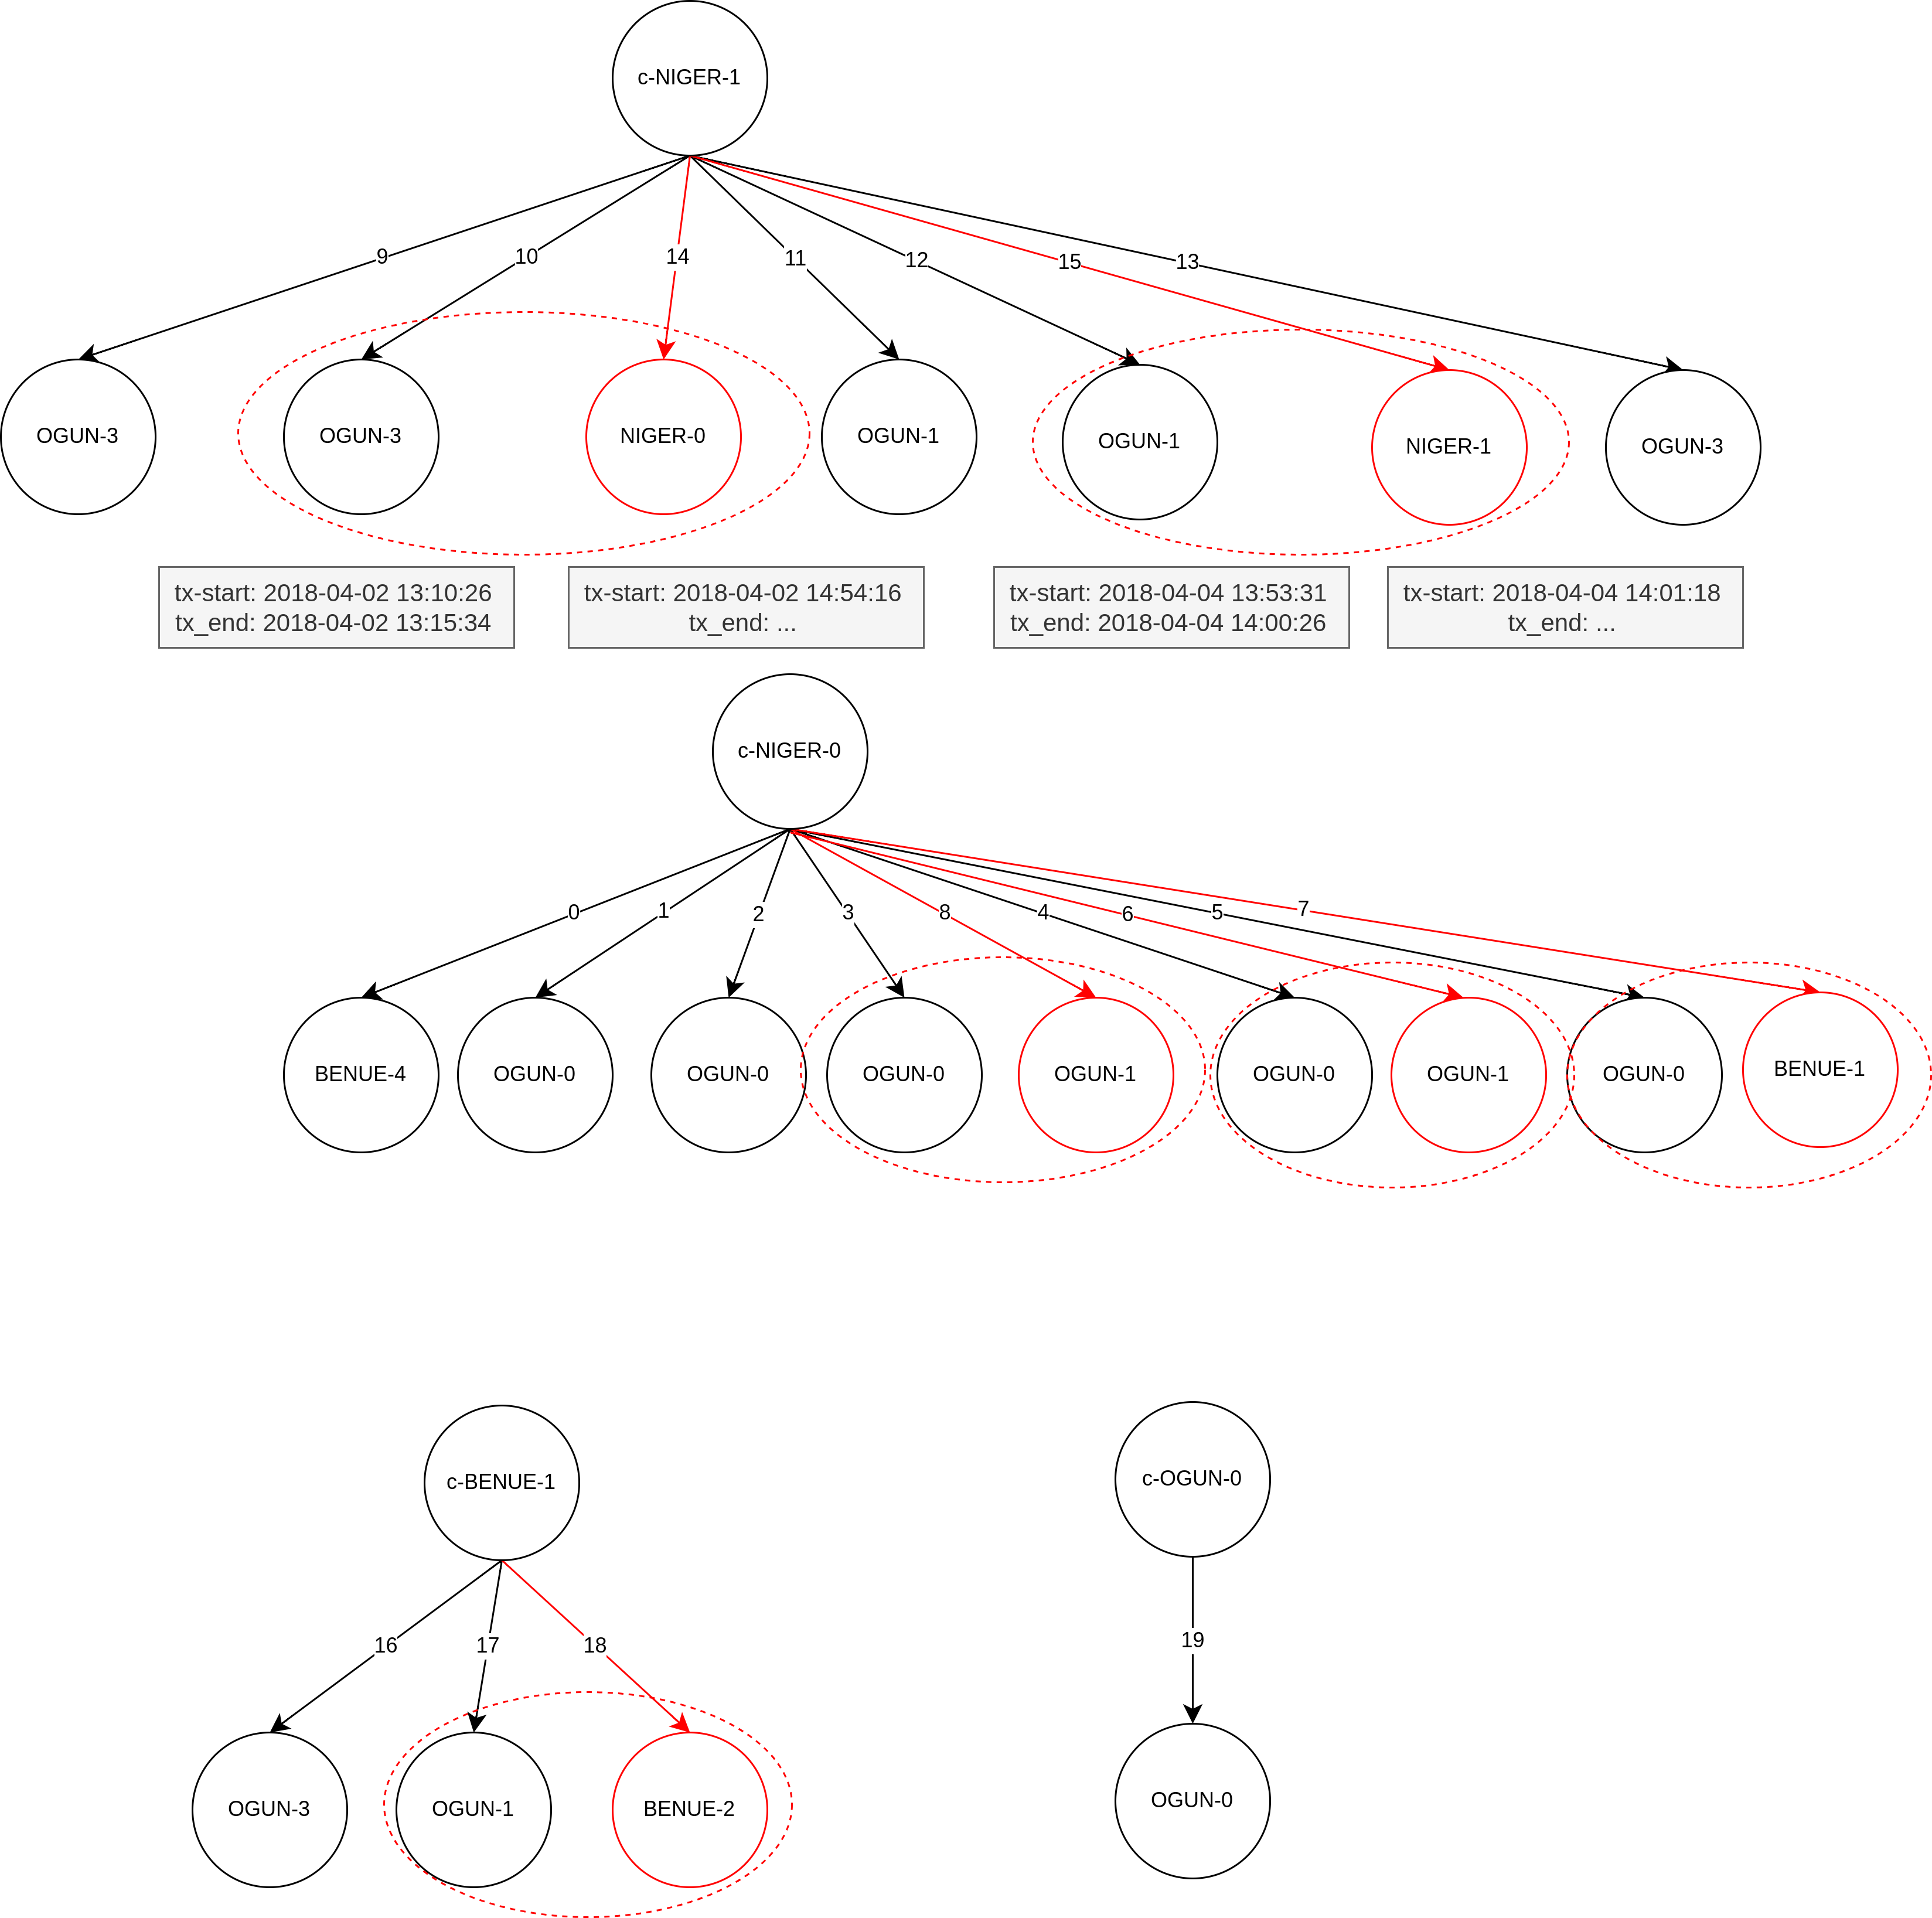
\includegraphics[scale=0.55]{images/2-QueryModel/FP1-test-1.png}
\end{figure}

\subsubsection{${FP}_1$ - Test 1.1}

\begin{figure}[H]
  \hspace*{-2cm} 
  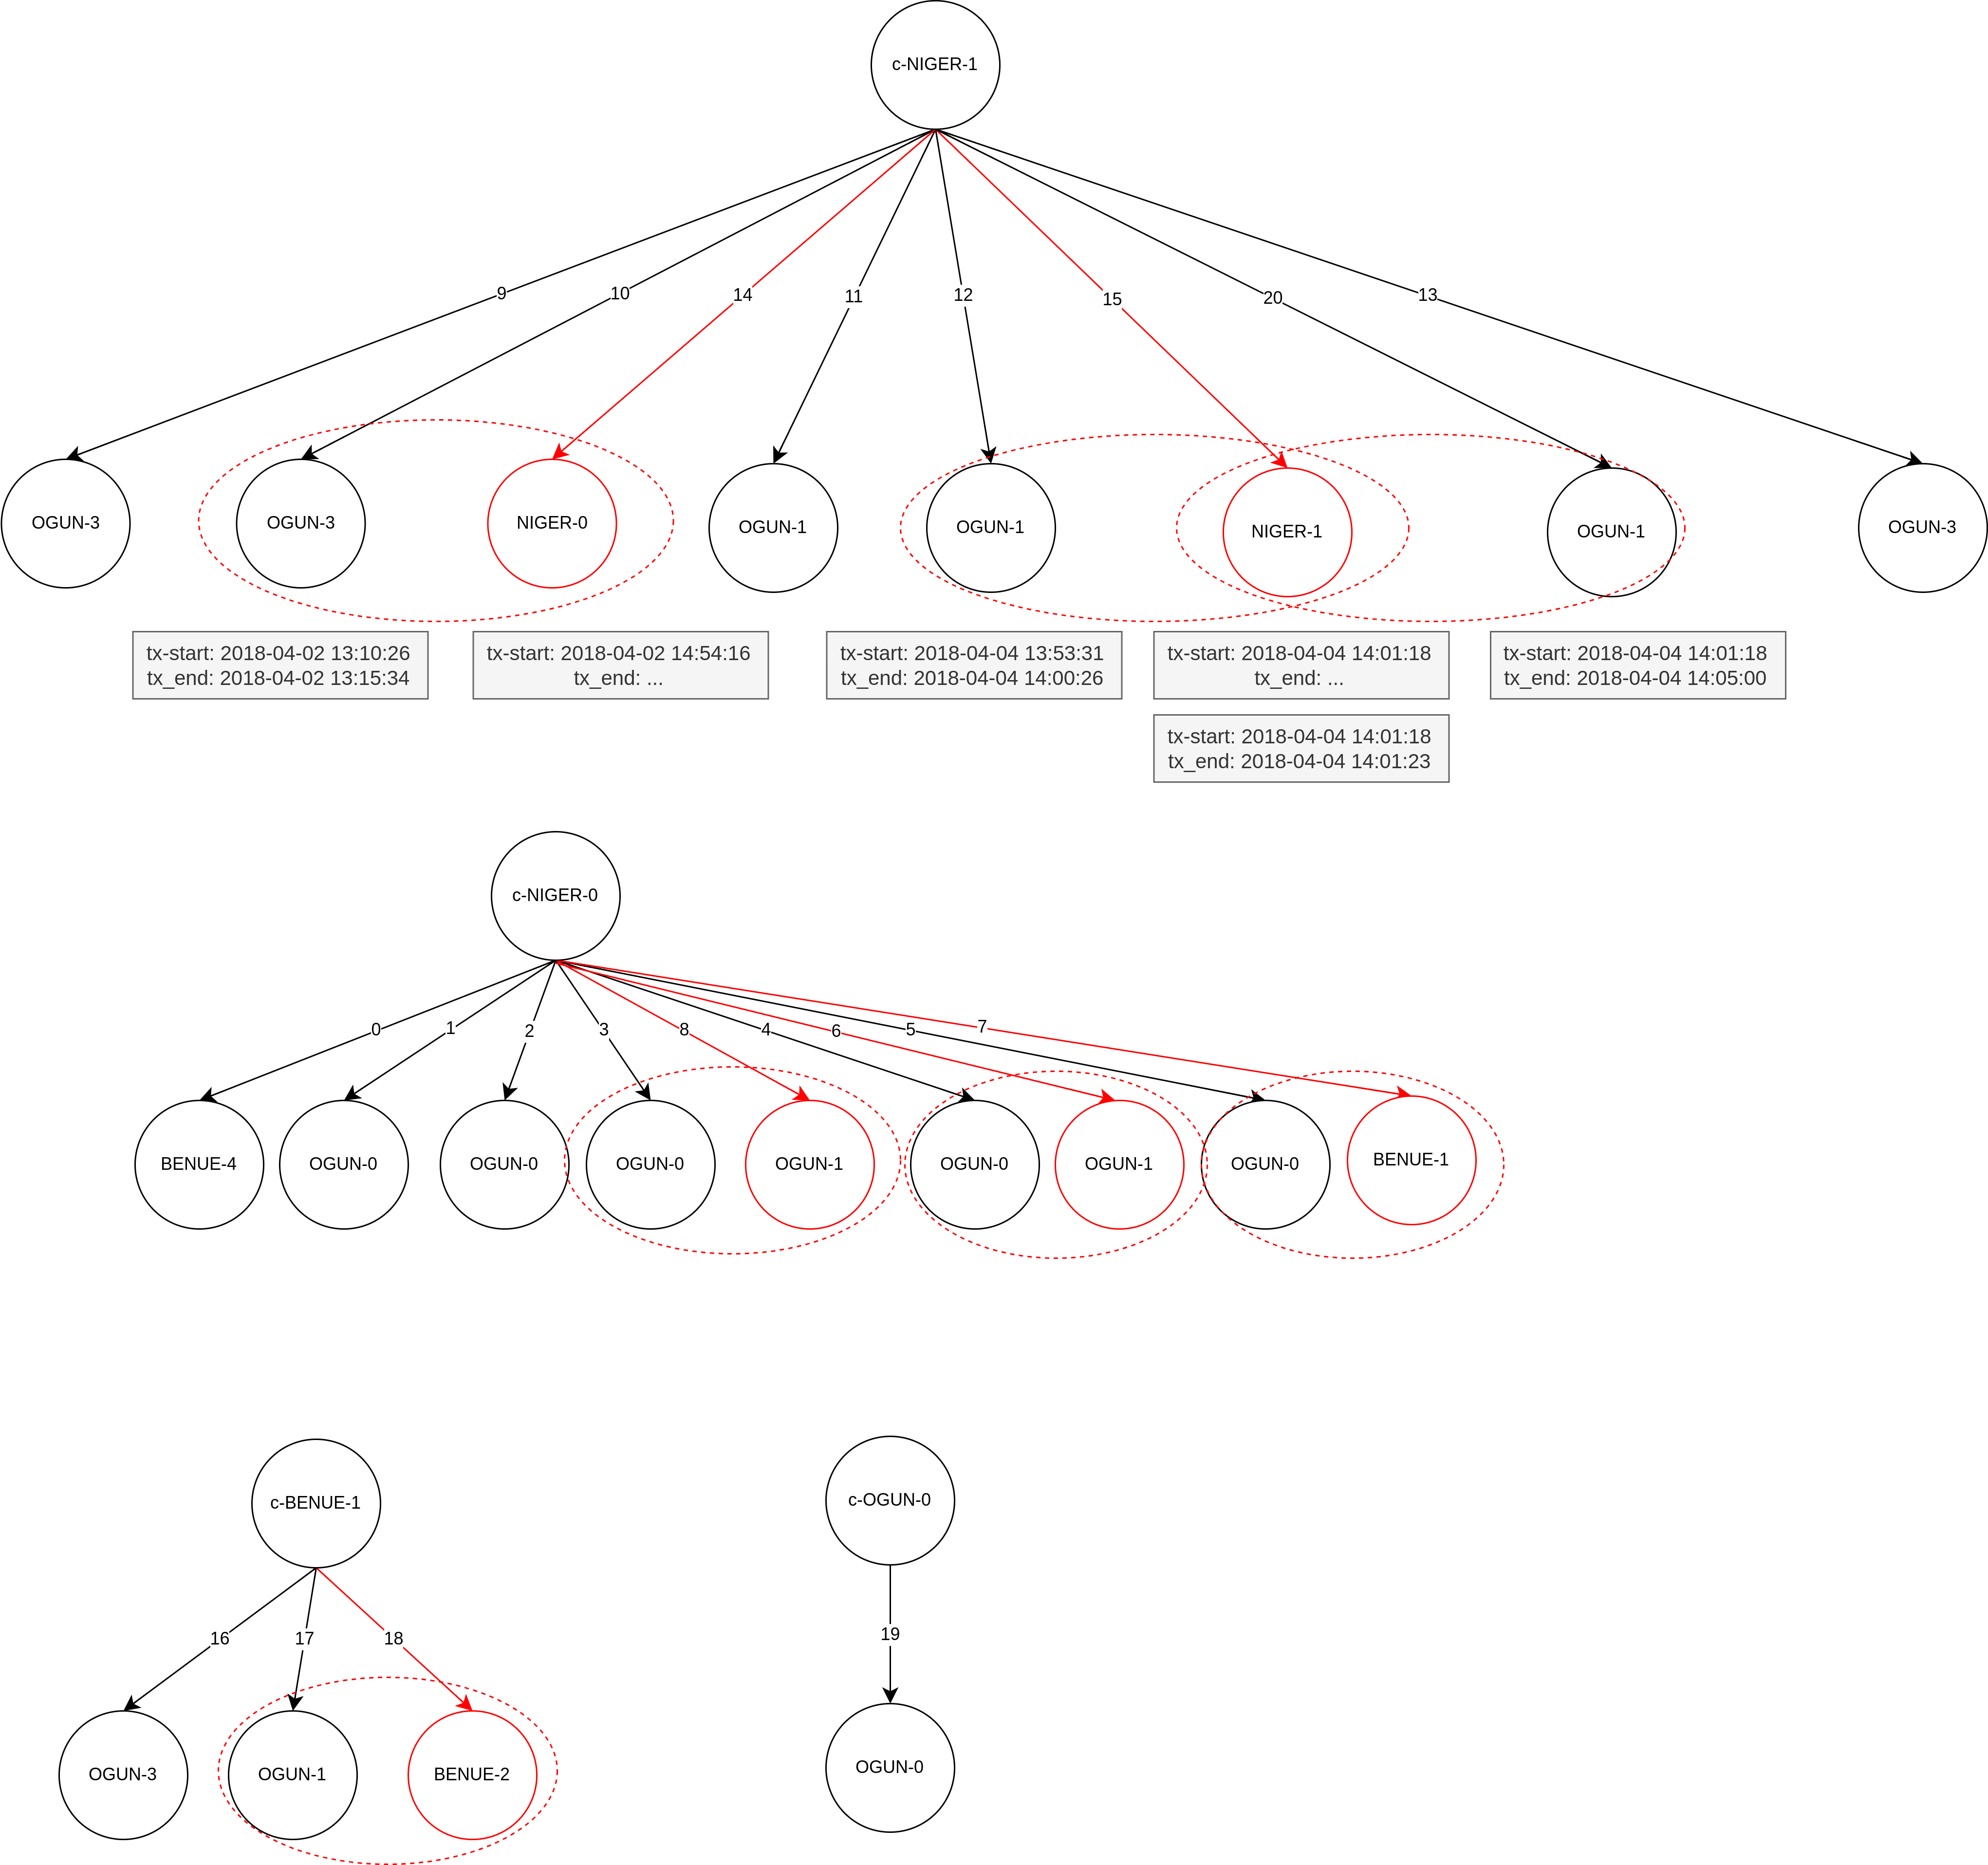
\includegraphics[scale=0.45]{images/2-QueryModel/FP1-test-1.1.png}
\end{figure}

\end{graysection}